


The script that solves the problem is \ttt{laplace.m} and is available at the end of the report with the subroutine \ttt{sol.m}. The boundary conditions in equation~\eqref{eq:cond2} are treated with ghost points. The conditions that the ghost point has the same value as the last point in the \textit{interior} of the domain. This is given by the discrete first derivative set to zero. 

Here is the output of our script. With figures~\ref{fig:h02} and~\ref{fig:h01}.

\begin{lstlisting}
>> laplace
T(2,1) = 450.000000 for h = 0.2 
T(2,1) = 450.000000 for h = 0.1
\end{lstlisting}

\begin{figure}[!h]
\centering
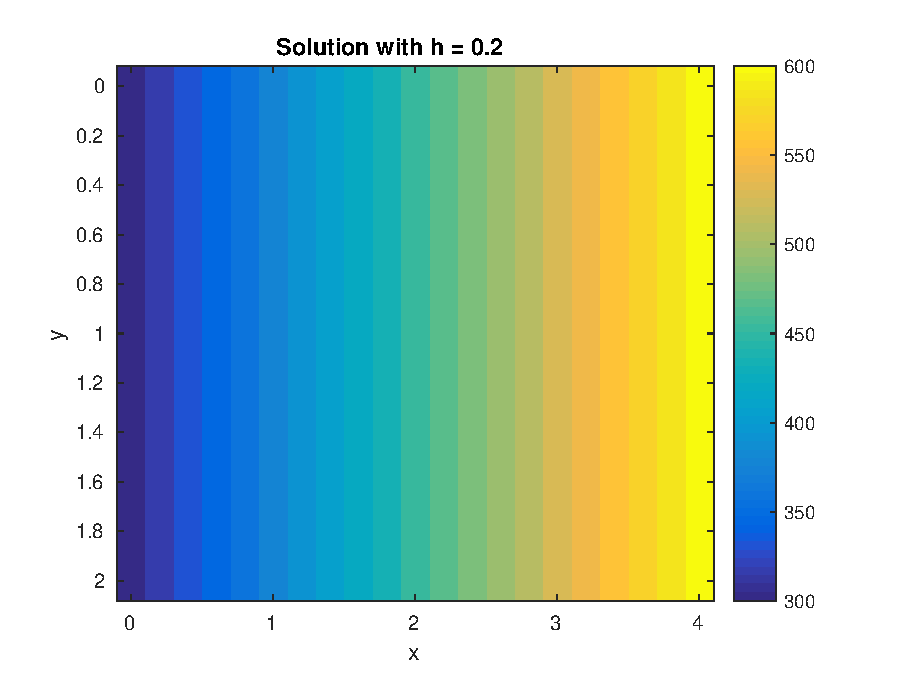
\includegraphics[width = 0.7\textwidth]{./h02.eps}
\caption{Solution with matlab for $h = 0.2$}
\label{fig:h02}
\end{figure}

\begin{figure}[!h]
\centering
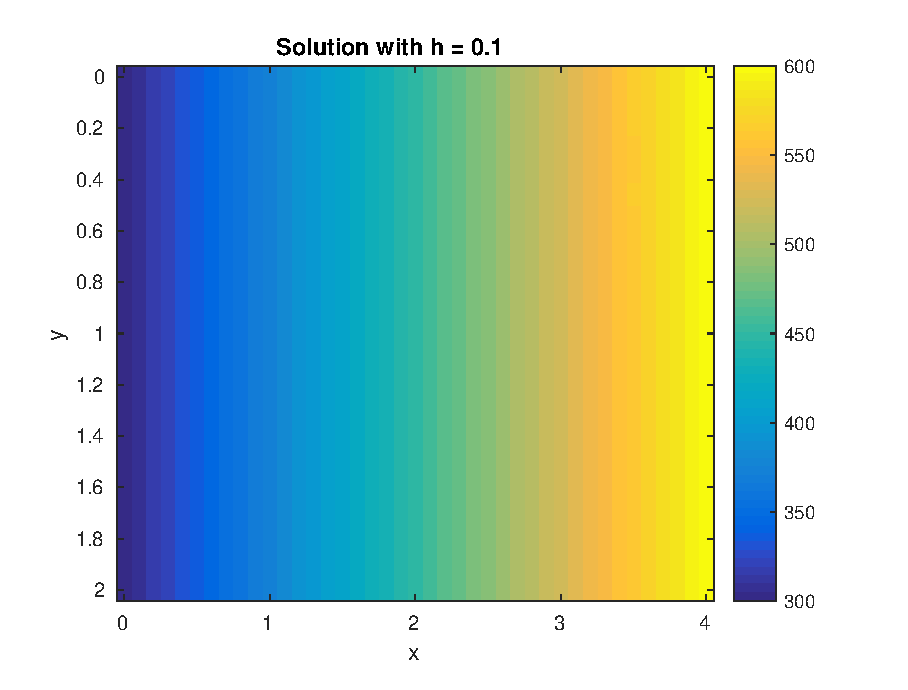
\includegraphics[width = 0.7\textwidth]{./h01.eps}
\caption{Solution with matlab for $h = 0.1$}
\label{fig:h01}
\end{figure}

\FloatBarrier
